\section{Discussion}
\label{sec:discussion}

\subsection{What is different about a millimetre technosignature search}
\label{sec:mmdifferent}

The most transferable result of this experiment is not the non-detection but
a measurement of what limits a carrier search at these wavelengths. For
classifying a crossing in the present archival data set, molecular-line
confusion and sparse repeat coverage are more immediate limitations than
thermal sensitivity. That is a statement about disposing of events and not
about depth: the power a transmitter must radiate to be found here remains a
median $\EirpNinetySysMedA$\,W per system.

\emph{Confusion, and not interference, sets the false-positive rate.}
Catalogued molecular transitions, almost all of them carbon monoxide, account
for \NAttributed{} of the \NCross{} threshold crossings, and no crossing in
this survey is attributed to interference (Appendix~\ref{app:rfi}).
\DiscFpWin{} of the \DiscFpOfFlags{} windows that reached the spatial stage
are disc or foreground carbon monoxide, arising in \DiscFpSys{} of the
\NDebrisKwSys{} debris-disc systems searched. The remedy that works is a
velocity-space mask evaluated in the stellar frame, and it is not free: it
removes \FrMaskPct{} per cent of otherwise usable coverage.

\emph{Spatially extended emission is the second discriminant, and it has no
analogue at centimetre wavelengths.} A line filling the primary beam raises
the star and the control annulus together instead of cancelling, so the
spatial statistic loses power exactly where circumstellar gas is brightest.
$\beta$~Pictoris shows the benign face: the frozen pipeline recovers its
circumstellar carbon monoxide blind, in two transitions, which is the positive
control the experiment needed. HD~48370 shows the other. Its resolved disc
emission lies near a band edge, and that one window contributes
\VnEdgeDomPct{} per cent of every near-edge threshold exceedance in the
survey: pooled, the near-edge rate is $\times\VnEdgeRatio$ the interior rate;
without that window $\times\VnEdgeNoDomRatio$, and on a held-out half
$\times\VnEdgeHalfCleanRatio$ ($\pv{\VnEdgeHalfCleanP}$). What looked like a
property of band edges is one disc, so no edge correction is applied to any
limit.

\emph{The channelisation is inherited.} \NCoarse{} of the \NWindows{} windows
have channels so coarse that every drift in the grid stays inside one channel
over a whole track; they measure an amplitude but cannot distinguish a
drifting carrier from a stationary one, which is why the carrier search rests
on \NWinA{} of them. The widths on offer here run from
\SzChanFinestKHz\,kHz to \SzChanWidestMHz\,MHz, about \SzChanDexSurvey{}
orders of magnitude; set beside the \SzChanLitHz\,Hz channels of
centimetre-band carrier searches the range becomes \SzChanDexAll{} orders
(Fig.~\ref{fig:context}(b)), and nothing in the search could choose them.

\emph{Repeat epochs turn a crossing into a testable claim, and an archive
supplies them only incidentally.} Let the \emph{confirmation coverage}
$C_{\rm conf}(\nu)$ be the number of systems toward which two independent
execution blocks more than a day apart both cover the sky frequency $\nu$, so
that a carrier found once there could have been sought again. It must be
stated against frequency rather than as a fraction of the sample, because
repeat visits re-tune and a second epoch is of no use at a frequency it does
not cover. Its support is \CvConfGHzDay\,GHz of union bandwidth,
\CvConfPctDay{} per cent of the \CvUnionA\,GHz searched, falling to
\CvConfGHzYr\,GHz beyond a year, and at its best near \CvConfNuMaxDay\,GHz it
reaches \CvConfNMaxDay{} systems (Fig.~\ref{fig:confcov}). The searched extent
is about twice the extent over which a persistent carrier could have been
confirmed, and for close to half the sample the archive constrains an
intermittent emitter hardly at all, whatever its power.

\begin{figure}
\centering
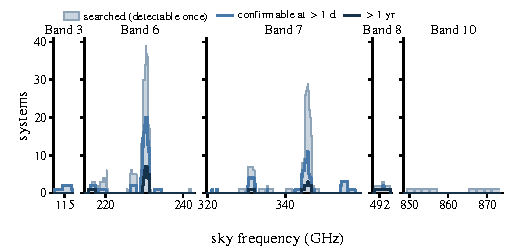
\includegraphics[width=\columnwidth]{figures/confcoverage.pdf}
\caption{What could be searched against what could be confirmed. For the
Class~A experiment, against sky frequency: the number of systems toward which
a carrier could have been detected once (grey), the number for which a second
independent execution block more than a day later also covers that frequency
(blue), and the same beyond a year (dark). One panel per populated ALMA band,
widths in proportion to the frequency each contributes, as in
Fig.~\ref{fig:covmap}.}
\label{fig:confcov}
\end{figure}

\emph{Finally, a threshold is not a sensitivity.} A trigger level is a
property of the noise, not of what a transmitter of a given power does to a
pipeline: measured by injection and recovery through the unchanged selection,
the power needed for ninety per cent recovery is $\EirpNinetyMultA$ times a
Class~A window's own trigger power and $\EirpNinetyMultB$ times a Class~B
window's.

\subsection{The search space this archive opens}
\label{sec:newspace}

The carrier search is \NWinA{} fine-channel windows toward \NSysClassA{}
stellar systems, \CvUnionA\,GHz of union bandwidth; the \NWinB{}
coarse-channel windows are a supplementary spectral-excess experiment. No previous search has looked for
technosignatures toward stars within 40\,pc above about 30\,GHz, and the one
earlier millimetre search worked in Band~3 toward far
more distant stars (\S\ref{sec:background}); Band~3 is searched here, in
\NWinBandThree{} windows down to \SurvFreqLo\,GHz including
$\beta$~Pictoris' CO $J=1\!-\!0$ control. Of the
\SttHayLoMHz\,MHz--\SttHayHiGHz\,GHz haystack axis of \citet{Wright2018} this
experiment covers \SttHayGHz\,GHz, only \SttHayFineGHz\,GHz of it carrier
search because the Class~A union begins at \SurvFreqLoA\,GHz; the rest lies
above that axis.

Union bandwidth overstates what that buys: different frequencies were searched
toward different numbers of stars and to very different
limits. Figure~\ref{fig:covmap} gives instead the number of independent systems
that would have yielded a recovery at ninety per cent completeness, against sky
frequency and transmitter power. At an
EIRP of $\CovEirpRefTex$\,W the covered frequency falls to
\CovUnionAtRef\,GHz, \CovFracAtRef{} per cent of the union, reaching
\CovNSysAtRef{} systems and \CovNMaxAtRef{} at the best-covered frequency near
\CovNuMaxAtRef\,GHz; with no limit on power that frequency reaches
\CovNMaxFull{} of the \NSysClassA{} systems, and half the sample only above
$\CovEirpHalf$\,W.

\begin{figure}
\centering
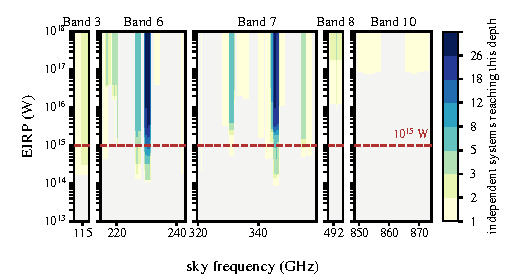
\includegraphics[width=\columnwidth]{figures/completeness_map.pdf}
\caption{Where the experiment could have found something. Shading gives the
number of independent systems that would have yielded a recovery at 90 per
cent completeness for an unresolved carrier of the plotted EIRP at the
plotted sky frequency; unshaded means none. One panel per populated ALMA
band, with panel widths in proportion to the frequency each contributes: the
\CvUnionA\,GHz Class~A union is \CovNIslands{} disjoint islands across
\DomAFreqLo--\DomAFreqHi\,GHz, which a continuous abscissa would draw as
hairlines. The dashed line is $\CovEirpRefTex$\,W.
Figure~\ref{fig:waterfall} shows where ALMA looked; this shows where the
experiment was sensitive.}
\label{fig:covmap}
\end{figure}

\emph{Archival SETI buys sky and frequency cheaply and buys confirmation not
at all}: \NSystems{} systems and \UnionGHz\,GHz of union bandwidth across both
classes without an allocation, on data selected by others and so carrying the
biases of \S\ref{sec:bias}.

The conventional measure for comparing programmes is the continuous-waveform
transmitter figure of merit of \citet{Enriquez2017},
$\mathrm{CWTFM}=\zeta_{\rm AO}\,\mathrm{EIRP}_{\rm min}/
(N_{\star}\nu_{\rm rel})$ with $\nu_{\rm rel}=\Delta\nu/\nu_{\rm mid}$,
smaller being better. Those programmes quote $\mathrm{EIRP}_{\rm min}$ at a
bare detection threshold, so the Class~A experiment is put on that footing:
with $N_{\star}=\NSysClassA$ and
$\nu_{\rm rel}=\FomNuRel$ it is $\SzCwtfmBareWorst$ on the sample's largest
threshold power and $\SzCwtfmBareMed$ on the median system, against
\FomLitEnriquez{} for that survey. \citet{Margot2023} publish no
CWTFM; the same expression on the three quantities they do give
--- \FomMargotN{} stars, \FomMargotLo--\FomMargotHi\,GHz and
$\mathrm{EIRP}>\FomMargotEirp$\,W --- returns \FomLitMargot.
With the $\mathrm{EIRP}_{90}$ adopted
everywhere else here the same two become $\FomCwtfmWorst$ and
$\FomCwtfmMed$. Nearly all of
the difference is the product $N_{\star}\nu_{\rm rel}$: this is a far smaller
haystack than a wideband centimetre survey of thousands of stars, and the
measure compares surveys rather than estimating occurrence rates.

\subsection{What this experiment excludes, and what it does not}
\label{sec:excludes}

\noindent\emph{Excluded.} Consider a continuously transmitting, unresolved
carrier that lies outside the molecular-line mask, inside the searched
frequency range and inside the linear-drift grid, and that is present during
one of the archival epochs. Such a carrier would have been found nine times
in ten above the $\mathrm{EIRP}_{90}$ of \S\ref{sec:pninetysel}, a median of
$\EirpNinetySysMedA$\,W per system on its best window. None was detected
toward any of the \NSysClassA{} systems the carrier search covers, at that
recovery probability and above that limit.

Four further axes bound the excluded population as sharply as power does.
\emph{Frequency:} the coverage is sparse and inherited (Fig.~\ref{fig:covmap})
and the median system is covered over only \SysUnionAMed\,GHz. \emph{Drift and
acceleration:} the grid reaches a line-of-sight acceleration of
\AccelCeilMed--\AccelCeilMax\,m\,s$^{-2}$, which contains every known planet
of the sample but one (Fig.~\ref{fig:accel}); an oscillator drifting faster
than that lies outside it. \emph{Persistence:} the carrier must be radiating
during one of the archival observations. \emph{Spectral width:} the statistic
is built for emission confined to one \ChanLoA--\ChanHiA\,kHz channel, and
anything broad enough to resemble continuum is removed with the spectral
baseline.

\noindent\emph{Not excluded.} A transmitter absent during the archival
observation, or on for much less than the length of one, at the cost in power
\S\ref{sec:pninetysel} measures. Emission inside the
$\pm\MaskHalfKms$\,km\,s$^{-1}$ molecular-line mask, at any strength, which
costs \FrMaskLostGHz\,GHz of union bandwidth. Drift outside the searched grid, or
drift curved enough to leave a channel within the track. Signals broad enough
to be removed with the continuum baseline. Anything below a window's own
completeness. And any emission from the \NGaiaCensus{} stars within 40\,pc
that ALMA has not observed, which is almost all of them.

\noindent\emph{An illustrative engineering benchmark.} A \BenchDiam\,m dish
radiating \BenchPowerMW\,MW at \BenchFreqGHz\,GHz with an aperture efficiency
of \BenchEta{} has a directive gain $G=\eta(\pi D\nu/c)^{2}=\BenchGain$ and so
an EIRP of $\BenchEirp$\,W, a depth this survey reaches for \BenchNSysA{} of
the \NSysClassA{} Class~A systems. The same gain fixes how narrow the beam is,
and detection requires the Earth to lie inside it: a solid angle
$\Omega=4\pi/G=\BmOmegaSr$\,sr, about \BmArcsec{} arcsec across, illuminating a
fraction $\Omega/4\pi=\BmSkyFrac$ of the sky at a time. The example shows that EIRP is not transmitter power --- the
same megawatt radiated isotropically would be $10^{6}$\,W --- so these limits
apply to beamed transmitters whose beam contains the Solar System and say
almost nothing about omnidirectional beacons.

\noindent\emph{Two blind spots.} The search is Stokes~$I$ only, so the
discrimination that polarisation would offer against unpolarised
astrophysical emission is unavailable; ALMA's feeds are linear, and the
circularity of a circularly polarised carrier lies in the cross-hands, which
this analysis does not extract. And the frequency coverage is the archive's
and not a choice: none of the ``magic frequency'' arguments that have guided
centimetre-band searches falls in an ALMA band, so a transmitter deliberately
placed on one lies outside this experiment by construction.

\subsection{What a dedicated ALMA technosignature experiment should do
differently}
\label{sec:future}

A purpose-built experiment on the same telescope would be far stronger, and
the changes it needs follow from the limitations above. \emph{Channelise
finely everywhere:} the \NCoarse{} coarse-channel windows cannot carry a
carrier search at all.
\emph{Choose the targets and the frequencies:} an archive weighted toward
dusty discs is the worst case for molecular-line confusion, the M~dwarfs that
dominate the nearby habitable-zone planet census are the least covered, and
windows placed deliberately away from the bright transitions would recover
most of the \FrMaskLostGHz\,GHz the mask costs --- all three are decisions a
proposal can simply reverse. \emph{Repeat the epochs on purpose, at the same
tuning:} two or three visits separated by days and by years turn a crossing
into a testable claim, and the separation is a scheduling constraint rather
than extra sensitivity; Fig.~\ref{fig:confcov} is what its absence costs.
\emph{Retain the visibilities:} rotating the phase centre to the star leaves a
genuine point source entirely in the real part of the visibility. That asks
whether the data contain a source \emph{where the star is}, which is a
stronger question than any rank
against neighbouring positions in an image.

%% ---------------------------------------------------------------------
%% REQUEST (06_discussion owner -> integrator). Consequences of this pass.
%% None of them is in a file I own; each is also written up as a numbered
%% entry in referee_r10/INTEGRATION_QUEUE.md.
%%
%% Q1. LABELS. sec:newspace, sec:excludes and sec:discussion are unchanged.
%%     sec:exposure and sec:parallax are GONE (see Q2, Q3); no file refers
%%     to either. sec:lessons is renamed sec:mmdifferent; the benchmark is
%%     a labelled paragraph inside sec:excludes, which is where \S2 now points.
%% Q2. THE OMITTED ANNUAL PARALLAX subsection is deleted from the Discussion
%%     under the ruling that the correction is applied rather than stated.
%%     The statement must now be made exactly once, where it is applied, in
%%     Section 5.1 / Appendix A. Macros \PxNWin, \PxLossMedPct,
%%     \PxLossMaxPct, \PxNGtTen and \PxNSysCorr are no longer referenced by
%%     any file I own and retire_macros.py will drop them unless that
%%     statement cites them.
%% Q3. THE ON-SOURCE TIME subsection (two offsetting bookkeeping biases) is
%%     deleted here as reproducibility detail. It belongs in Appendix A.
%%     Macros \TruncNBlocks, \ExpNBlocks, \TruncNWin, \TruncNStars,
%%     \TruncHoursLost, \TruncPctSurvey, \TruncGainMed, \OcOldMax,
%%     \OcNewMax, \ExpNetLo, \ExpNetHi are orphaned by that deletion.
%% Q4. THE MASON MATCHED-RECEIVED-FLUX COMPARISON is now made once, in
%%     Section 2, as that section's own request asked. \FluxSelMatchMed and
%%     \FluxSelMedRatio are unused.
%% Q5. THE BENCHMARK must stop being quoted as a headline result elsewhere:
%%     it is now an explicitly illustrative example in Section 6.3.
%%     Remove it from the abstract, from Section 5 and from conclusion 3,
%%     each of which should quote the EIRP_90 limit alone.
%% Q6. CONCLUSION 1 states that \UnionBandThree GHz of the searched range
%%     lies inside the interval covered by centimetre-wave programmes. It
%%     does not; that is the Band 3 union inside the Wright et al. haystack
%%     AXIS. Replacement text is in the integration queue.
%% Q7. Figure fig:covmap is new and is paid for: the millimetre-motivation
%%     paragraph (duplicated from Section 1), the Mason flux comparison, the
%%     parallax subsection and the exposure subsection are all deleted here.
%% ---------------------------------------------------------------------
